\documentclass{ximera}

%% You can put user macros here
%% However, you cannot make new environments

\listfiles

\graphicspath{{./}{firstExample/}{secondExample/}}

\usepackage{tikz}
\usepackage{tkz-euclide}
\usepackage{tikz-3dplot}
\usepackage{tikz-cd}
\usetikzlibrary{shapes.geometric}
\usetikzlibrary{arrows}
\usetikzlibrary{decorations.pathmorphing,patterns}
\usetkzobj{all}
\pgfplotsset{compat=1.13} % prevents compile error.

\renewcommand{\vec}[1]{\mathbf{#1}}
\newcommand{\RR}{\mathbb{R}}
\newcommand{\dfn}{\textit}
\newcommand{\dotp}{\cdot}
\newcommand{\id}{\text{id}}
\newcommand\norm[1]{\left\lVert#1\right\rVert}
 
\newtheorem{general}{Generalization}
\newtheorem{initprob}{Exploration Problem}

\tikzstyle geometryDiagrams=[ultra thick,color=blue!50!black]

\usepackage{mathtools}

\title{Convolution}%\label{Module 7-ADEF}


\begin{document}

\begin{abstract}
We define the convolution of two functions, and discuss its application to computing the inverse Laplace transform of a product.
\end{abstract}

\maketitle

\section*{Convolution}

In this section we consider the problem of finding the inverse Laplace
transform of a product $H(s)=F(s)G(s)$, where $F$ and $G$ are the
Laplace transforms of known functions $f$ and $g$. To motivate our
interest in this problem, consider the initial value problem
$$
ay''+by'+cy=f(t),\quad y(0)=0,\quad y'(0)=0.
$$
Taking Laplace transforms  yields
$$
(as^2+bs+c)Y(s)=F(s),
$$
so
\begin{equation}\label{eq:8.6.1}
Y(s)=F(s)G(s),
\end{equation}
where
$$
G(s)=\frac{1}{as^2+bs+c}.
$$

Until now haven't been interested in the factorization indicated
in \eqref{eq:8.6.1}, since we dealt only with differential equations
with specific forcing functions. Hence, we could simply do the
indicated multiplication in \eqref{eq:8.6.1} and use the table of Laplace
transforms to find $y={\cal L}^{-1}(Y)$. However, this isn't  possible
if we want a \textit{formula} for $y$ in terms of $f$, which may be
unspecified.

To motivate the formula for ${\cal L}^{-1}(FG)$, consider the initial
value problem
\begin{equation}\label{eq:8.6.2}
y'-ay=f(t),\quad  y(0)=0,
\end{equation}
which we first solve without using the Laplace transform.
The solution of  the differential equation in \eqref{eq:8.6.2}
is of the form $y=ue^{at}$ where
$$
u'=e^{-at}f(t).
$$
Integrating this from $0$ to $t$ and imposing the initial condition
$u(0)=y(0)=0$ yields
$$
u=\int_0^t e^{-a\tau}f(\tau)\,d\tau.
$$
Therefore
\begin{equation}\label{eq:8.6.3}
y(t)=e^{at}\int_0^t e^{-a\tau}f(\tau)\,d\tau=\int_0^t
e^{a(t-\tau)}f(\tau)\,d\tau.
\end{equation}

Now we'll use the Laplace transform to solve \eqref{eq:8.6.2}
and compare the result to \eqref{eq:8.6.3}. Taking Laplace transforms in
\eqref{eq:8.6.2} yields
$$
(s-a)Y(s)=F(s),
$$
so
$$
Y(s)=F(s) \frac{1}{s-a},
$$
which implies that
\begin{equation}\label{eq:8.6.4}
y(t)= {\cal L}^{-1}\left(F(s)\frac{1}{s-a}\right).
\end{equation}
If we now let $g(t)=e^{at}$, so that
$$
G(s)=\frac{1}{s-a},
$$
then \eqref{eq:8.6.3} and \eqref{eq:8.6.4} can be written as
$$
y(t)=\int_0^tf(\tau)g(t-\tau)\,d\tau
$$
and
$$
y={\cal L}^{-1}(FG),
$$
respectively.  Therefore
\begin{equation}\label{eq:8.6.5}
{\cal L}^{-1}(FG)=\int_0^t f(\tau)g(t-\tau)\,d\tau
\end{equation}
in this case.

This motivates  the next definition.

\begin{definition}\label{thmtype:8.6.1}
The \textit{convolution} $f\ast g$ of two functions $f$
and $g$ is defined by
$$
(f\ast g)(t)=\int_0^t f(\tau)g(t-\tau)\,d\tau.
$$
\end{definition}

It can be shown %(Exercise~\ref{exer:8.6.6}) 
that $f\ast g=g\ast f$;   that
is,
$$
\int_0^tf(t-\tau)g(\tau)\,d\tau=\int_0^tf(\tau)g(t-\tau)\,d\tau.
$$

Eqn.~\eqref{eq:8.6.5} shows that ${\cal L}^{-1}(FG)=f\ast g$ in the special
case where $g(t)=e^{at}$. This next theorem states that this is
true in general.

\begin{theorem}[The Convolution
Theorem]\label{thmtype:8.6.2}
If ${\cal L}(f)=F$  and ${\cal L}(g)=G,$ then
$$
{\cal L}(f\ast g)=FG.
$$
\end{theorem}

A complete proof of the convolution theorem is beyond the scope of
this book. However, we'll assume that $f\ast g$ has a Laplace
transform and verify the conclusion of the theorem in a purely
computational way. By the definition of the Laplace transform,
$$
{\cal L}(f\ast g)=\int_0^\infty e^{-st}(f\ast g)(t)\,dt=\int_0^\infty
e^{-st}
\int_0^t f(\tau)g(t-\tau)\,d\tau\,dt.
$$
This iterated integral equals a double integral over the region shown
in %Figure~\ref{figure:8.6.1}. 
the figure below.

\begin{image}
 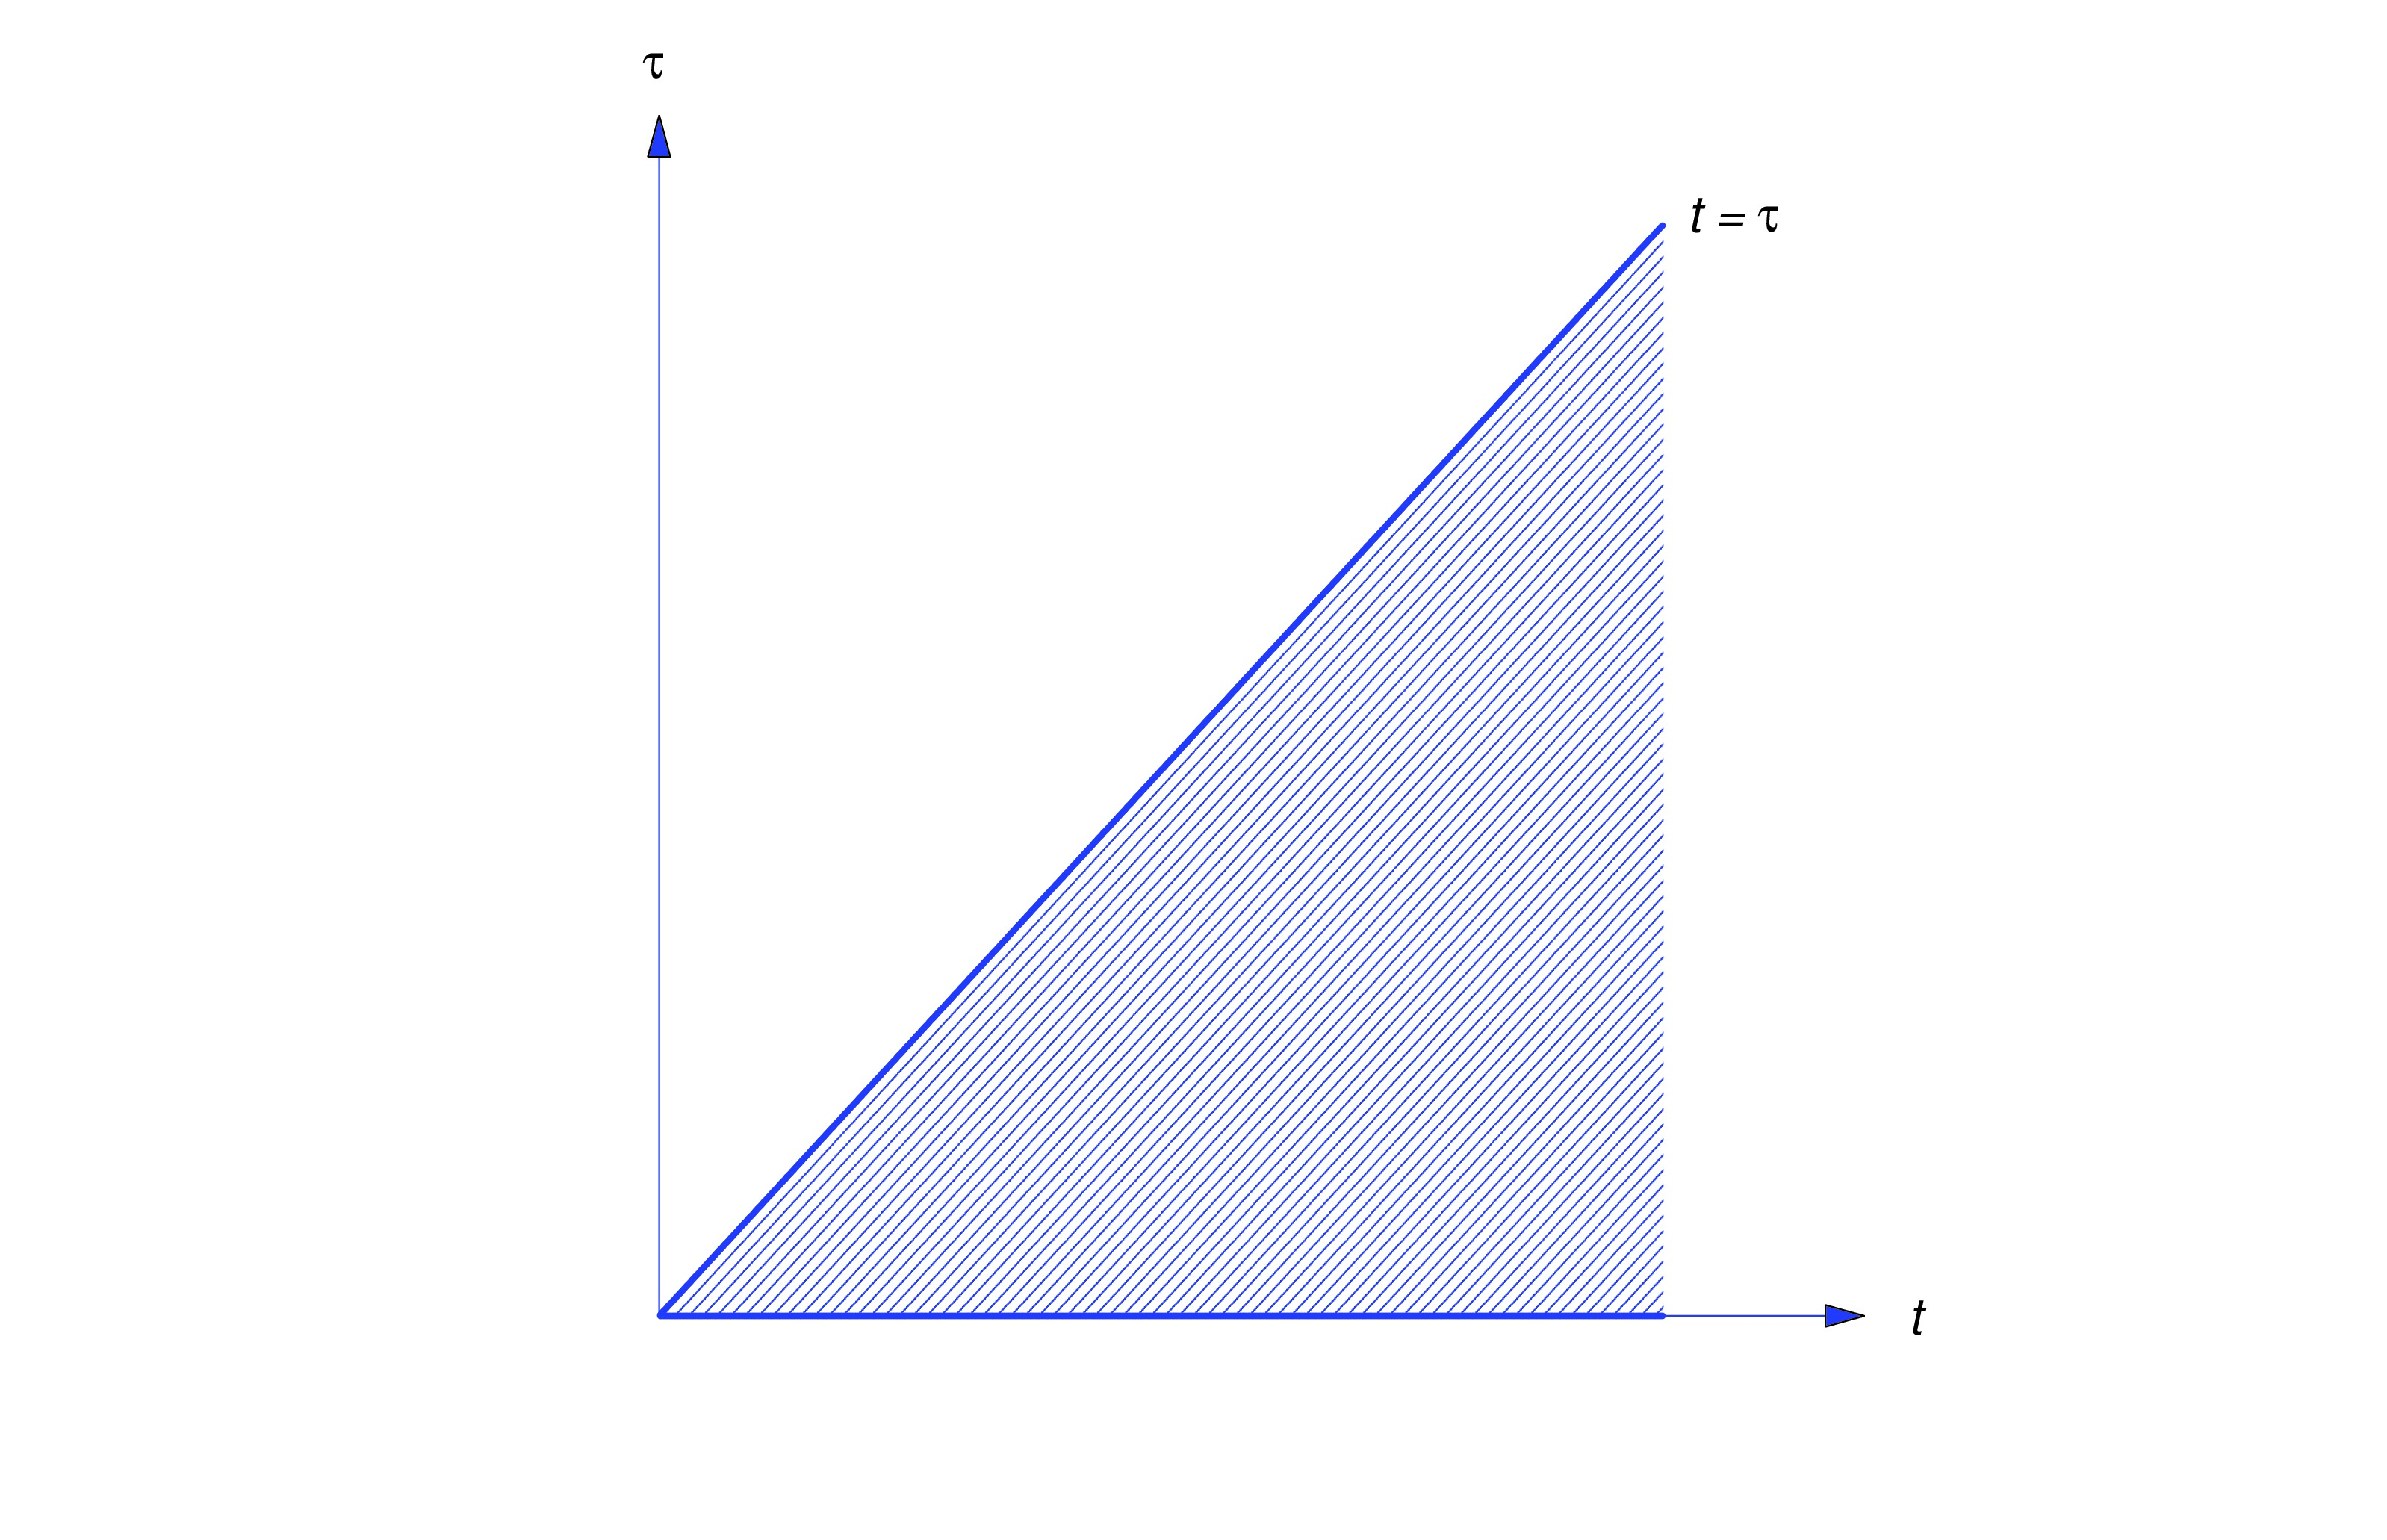
\includegraphics[height=1.5in]{fig080601.jpg} 
\end{image}

Reversing the order of integration yields
\begin{equation}\label{eq:8.6.6}
{\cal L}(f\ast g)=\int_0^\infty f(\tau)\int^\infty_\tau e^{-st}g(t-\tau)\,
dt
\,d\tau.
\end{equation}
However, the substitution $x=t-\tau$ shows that
\begin{eqnarray*}
\int^\infty_\tau e^{-st}g(t-\tau)\,dt&=&\int_0^\infty
e^{-s(x+\tau)}g(x)\,dx\\
&=&e^{-s\tau}\int_0^\infty e^{-sx}g(x)\,dx=e^{-s\tau}G(s).
\end{eqnarray*}
Substituting this into  \eqref{eq:8.6.6} and noting that $G(s)$ is
independent of $\tau$ yields
\begin{eqnarray*}
{\cal L}(f\ast g)&=&\int_0^\infty e^{-s\tau} f(\tau)G(s)\,d\tau\\
&=&G(s)\int_0^\infty e^{-st}f(\tau)\,d\tau=F(s)G(s).
\end{eqnarray*}

% \
% \begin{figure}[tbp]
%   \centering\color{blue}
%   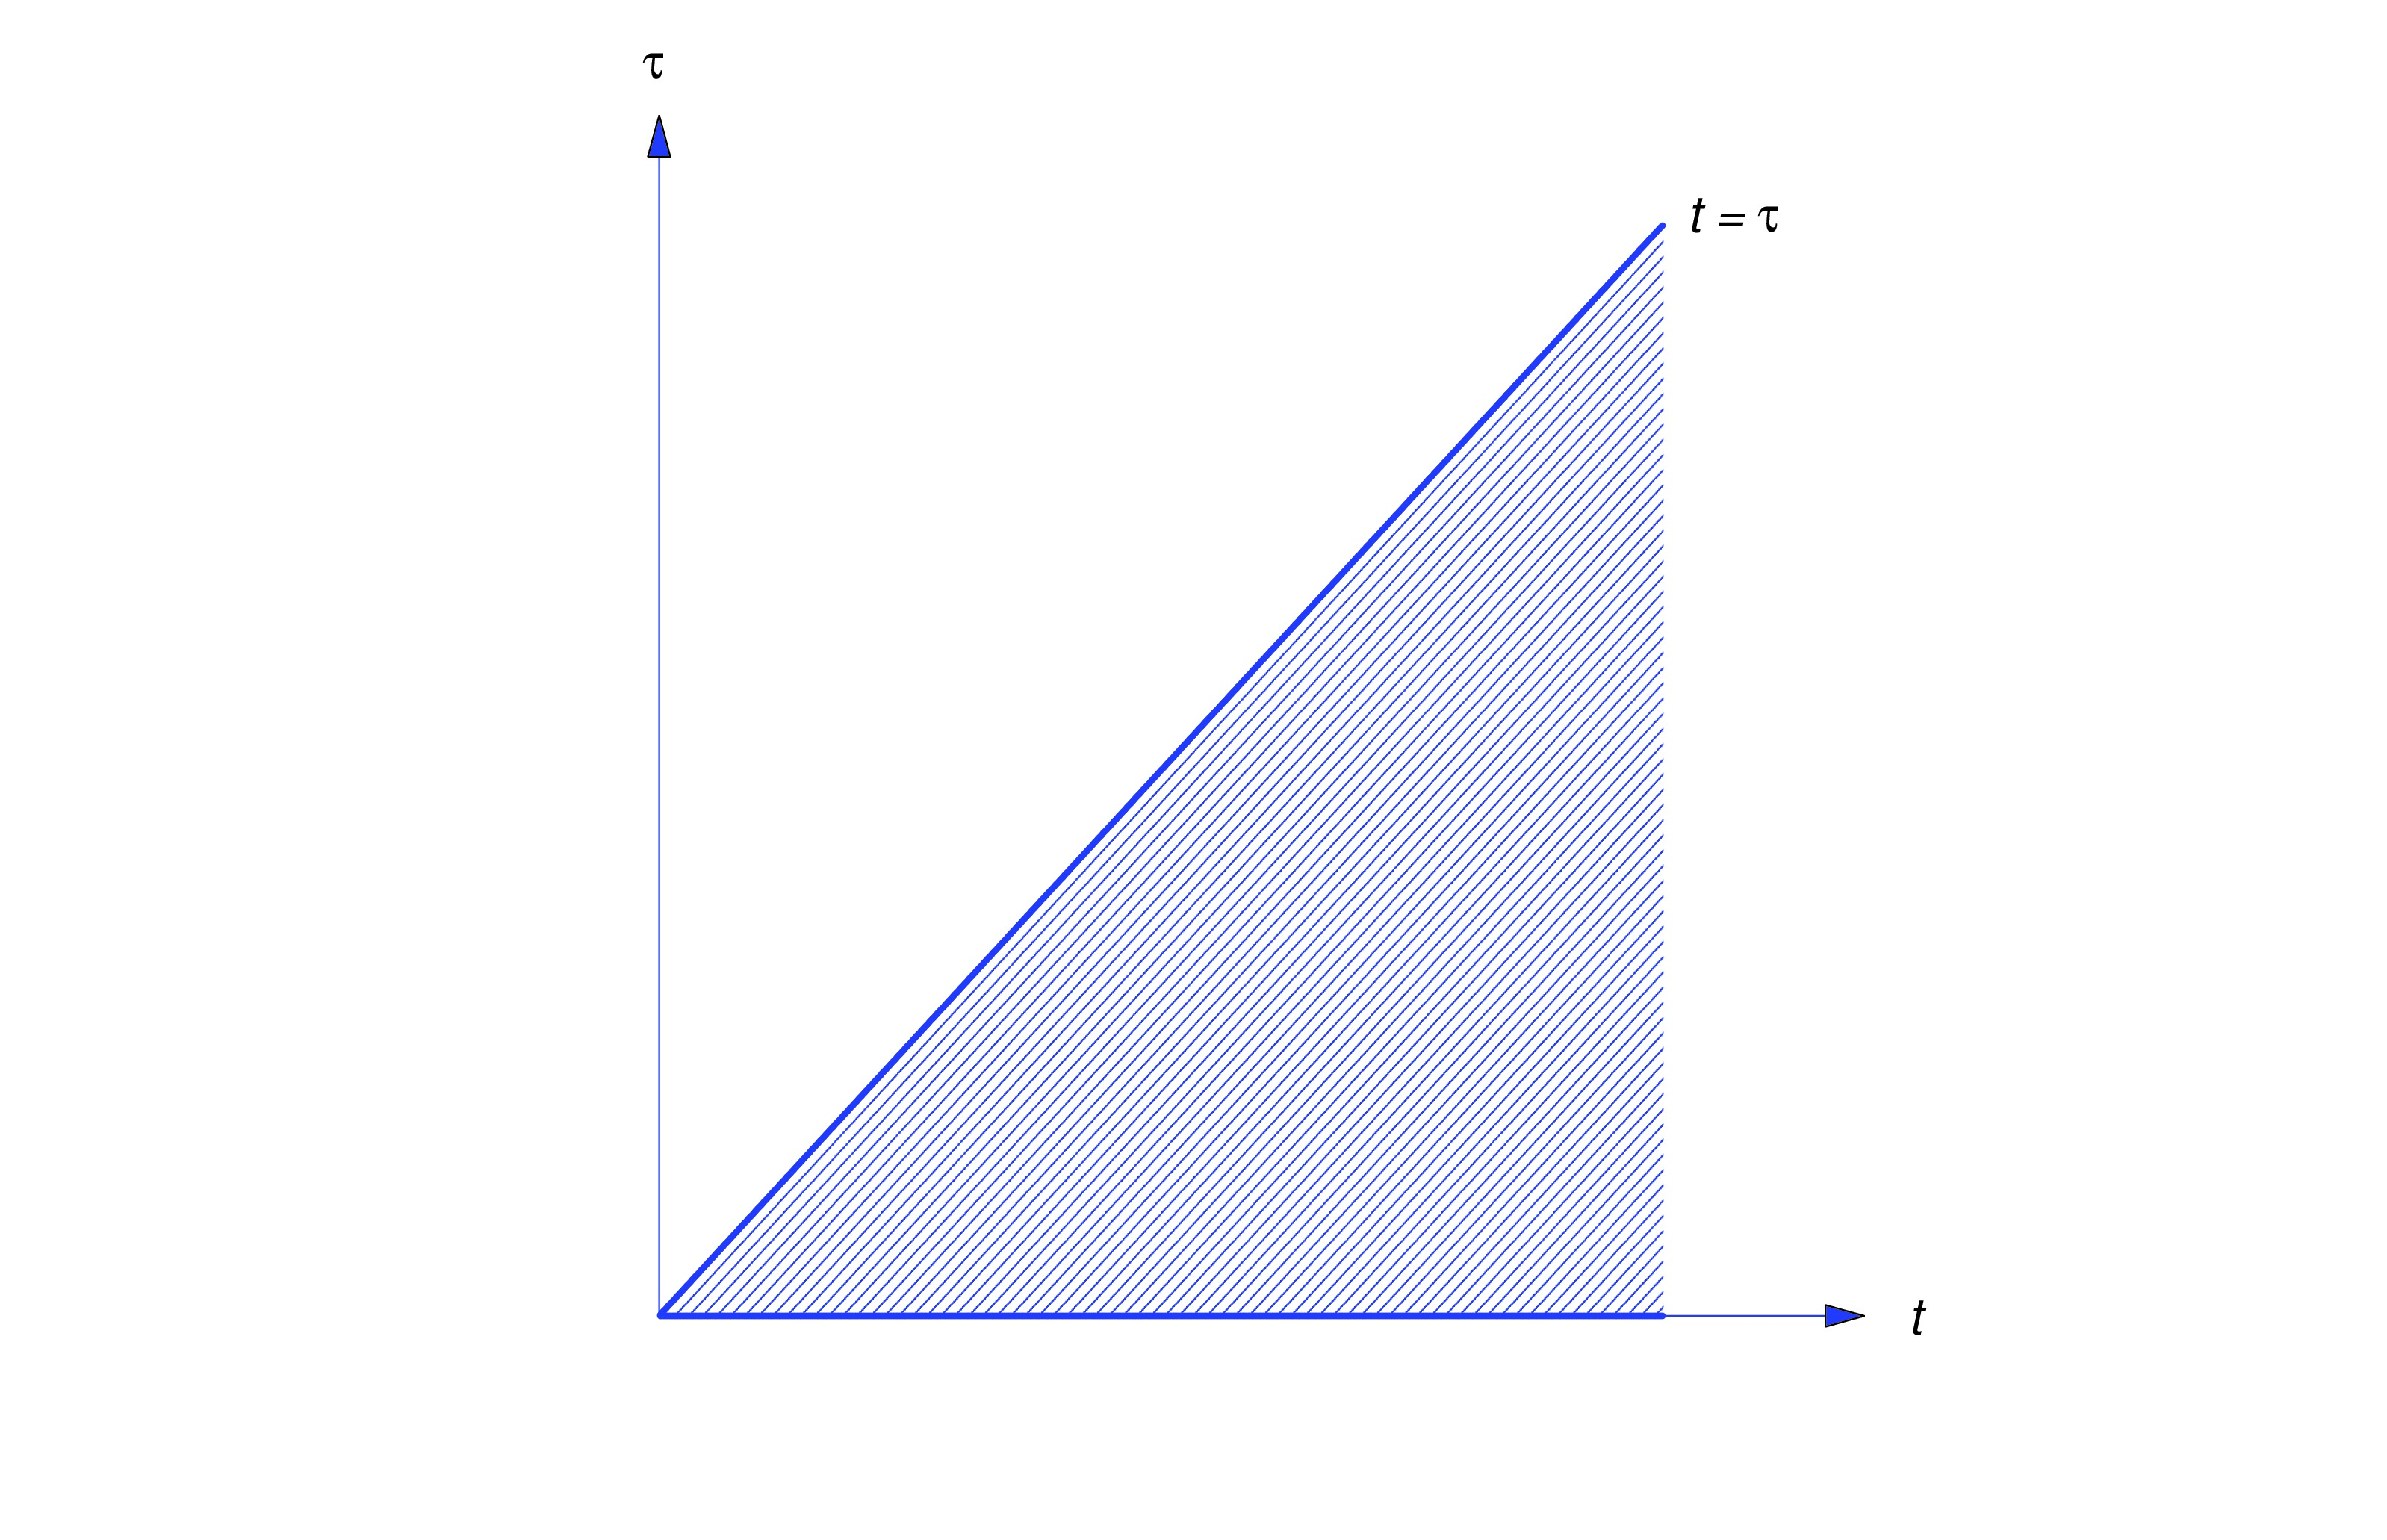
\includegraphics[bb=-78 148 689 643,width=5.67in,height=3.66in,keepaspectratio]{fig080601}
%   \caption{}
%   \label{figure:8.6.1}
% \end{figure}

\begin{example}\label{example:8.6.1}
 Let
$$
f(t)=e^{at}\quad\mbox{and}\quad  g(t)=e^{bt}\qquad (a\ne b).
$$
Verify that ${\cal L}(f\ast g)={\cal L}(f){\cal L}(g)$, as
implied by the convolution theorem.
\begin{explanation}
We first compute
$$
\begin{array}{ccccc}
(f\ast g)(t)&=&\int_0^t e^{a\tau}e^{b(t-\tau)}\,d\tau
&=&e^{bt}\int_0^t e^{(a-b)\tau} d\tau\\
&=&e^{bt} \frac{e^{(a-b)\tau}}{ a-b}\,\bigg|^t_0&=&
e^{bt}\frac{\left[e^{(a-b)t}-1\right]}{a-b}\\
&=&\frac{e^{at}-e^{bt}}{a-b}.
\end{array}
$$
Since
$$
e^{at}\leftrightarrow \frac{1}{s-a}\quad\mbox{and}\quad
e^{bt}\leftrightarrow \frac{1}{s-b},
$$
it follows that
\begin{eqnarray*}
{\cal L}(f\ast g)&=&\frac{1}{a-b}\left[\frac{1}{s-a}-\frac{1}{s-b}\right]\\
&=&\frac{1}{(s-a)(s-b)}\\
&=&{\cal L}(e^{at}){\cal L}(e^{bt})={\cal L}(f){\cal L}(g).
\end{eqnarray*}
\end{explanation}
\end{example}

\subsection*{A Formula for the Solution of an Initial Value Problem}

The convolution theorem provides a formula for the
solution of an initial value problem for a linear constant coefficient
second order equation with an unspecified set of initial conditions.
The next three examples illustrate this.

\begin{example}\label{example:8.6.2}
 Find a formula for the solution of the initial value problem
\begin{equation}\label{eq:8.6.7}
y''-2y'+y=f(t),\quad  y(0)=k_0,\quad y'(0)=k_1.
\end{equation}
\begin{explanation}
Taking Laplace transforms in \eqref{eq:8.6.7} yields
$$
(s^2-2s+1)Y(s)=F(s)+(k_1+k_0s)-2k_0.
$$
Therefore
\begin{eqnarray*}
Y(s)&=&\frac{1}{(s-1)^2}F(s)+\frac{k_1+k_0s-2k_0}{(s-1)^2}\\
&=&\frac{1}{(s-1)^2}F(s)+\frac{k_0}{s-1}+\frac{k_1-k_0}{(s-1)^2}.
\end{eqnarray*}
From the table of Laplace transforms,
$$
{\cal L}^{-1}\left(\frac{k_0}{s-1}+\frac{k_1-k_0}{(s-1)^2}\right)
=e^t\left(k_0+(k_1-k_0)t\right).
$$
Since
$$
\frac{1}{(s-1)^2}\leftrightarrow te^t\quad\mbox{and}\quad F(s)
\leftrightarrow f(t),
$$
the convolution theorem implies that
$$
{\cal L}^{-1}
\left(\frac{1}{(s-1)^2}F(s)\right)=
\int_0^t\tau e^\tau f(t-\tau)\,d\tau.
$$
Therefore the solution of  \eqref{eq:8.6.7} is
$$
y(t)=e^t\left(k_0+(k_1-k_0)t\right)+\int_0^t\tau e^\tau f(t-\tau)\,
d\tau.
$$
\end{explanation}
\end{example}

\begin{example}\label{example:8.6.3}
 Find a formula for the solution of the initial value problem
\begin{equation}\label{eq:8.6.8}
y''+4y=f(t),\quad y(0)=k_0,\quad y'(0)=k_1.
\end{equation}
\begin{explanation}
Taking Laplace transforms in \eqref{eq:8.6.8} yields
$$
(s^2+4)Y(s) =F(s)+k_1+k_0s.
$$
Therefore
$$
Y(s) =\frac{1}{(s^2+4)}F(s)+\frac{k_1+k_0s}{s^2+4}.
$$
From the table of Laplace transforms,
$$
{\cal L}^{-1}\left(\frac{k_1+k_0s}{s^2+4}\right)=k_0\cos 2t+\frac{k_1}{2}\sin 2t.
$$
Since
$$
\frac{1}{(s^2+4)}\leftrightarrow \frac{1}{2}\sin 2t\quad\mbox{and}\quad
F(s)\leftrightarrow f(t),
$$
the convolution theorem implies that
$$
{\cal L}^{-1}\left(\frac{1}{(s^2+4)}F(s)\right)=
 \frac{1}{2}\int_0^t  f(t-\tau)\sin 2\tau\,
d\tau.
$$
Therefore the solution of  \eqref{eq:8.6.8} is
$$
y(t)=k_0\cos 2t+\frac{k_1}{2}\sin 2t+\frac{1}{2}\int_0^tf(t-\tau)\sin
2\tau\,d\tau.
$$
\end{explanation}
\end{example}

\begin{example}\label{example:8.6.4}
  Find a formula for the solution of the initial value problem
\begin{equation}\label{eq:8.6.9}
y''+2y'+2y=f(t),\quad y(0)=k_0,\quad y'(0)=k_1.
\end{equation}
\begin{explanation}
Taking Laplace transforms in \eqref{eq:8.6.9} yields
$$
(s^2+2s+2)Y(s)=F(s)+k_1+k_0s+2k_0.
$$
Therefore
\begin{eqnarray*}
Y(s)&=&\frac{1}{(s+1)^2+1}F(s)+\frac{k_1+k_0s+2k_0}{(s+1)^2+1}\\
&=&\frac{1}{(s+1)^2+1}F(s)+\frac{(k_1+k_0)+k_0(s+1)}{(s+1)^2+1}.
\end{eqnarray*}
From the table of Laplace transforms,
$$
{\cal L}^{-1}\left(\frac{(k_1+k_0)+k_0(s+1)}{(s+1)^2+1}\right)=
e^{-t}\left((k_1+k_0)\sin t+k_0\cos t\right).
$$
Since
$$
\frac{1}{(s+1)^2+1}\leftrightarrow e^{-t}\sin t\quad\mbox{and}\quad
 F(s)\leftrightarrow f(t),
$$
the convolution theorem implies that
$$
{\cal L}^{-1}\left(\frac{1}{(s+1)^2+1}F(s)\right)=
\int_0^t  f(t-\tau)e^{-\tau}\sin\tau
\,d\tau.
$$
Therefore the solution of  \eqref{eq:8.6.9} is
\begin{equation}\label{eq:8.6.10}
y(t)=e^{-t}\left((k_1+k_0)\sin t+k_0\cos
t\right)+\int_0^tf(t-\tau)e^{-\tau}\sin\tau\,d\tau.
\end{equation}
\end{explanation}
\end{example}

\subsection*{Evaluating Convolution Integrals}

We'll say that an integral of the form $\int_0^t
u(\tau)v(t-\tau)\,d\tau$ is a \textit{convolution integral}. The
convolution theorem provides a convenient way to evaluate convolution
integrals.

\begin{example}\label{example:8.6.5}
 Evaluate the convolution integral
$$
h(t)=\int_0^t(t-\tau)^5\tau^7 d\tau.
$$
\begin{explanation}
We could evaluate this integral by expanding
$(t-\tau)^5$ in powers of $\tau$ and then integrating. However, the
convolution theorem provides an easier way. The integral is the
convolution of $f(t)=t^5$ and $g(t)=t^7$. Since
$$
t^5\leftrightarrow \frac{5!}{s^6}\quad\mbox{and}\quad  t^7
\leftrightarrow \frac{7!}{s^8},
$$
the convolution theorem implies that
$$
h(t)\leftrightarrow \frac{5!7!}{s^{14}}=\frac{5!7!}{13!}\, \frac{13!}{s^{14}},
$$
where we have written the second equality because
$$
\frac{13!}{ s^{14}}\leftrightarrow t^{13}.
$$
Hence,
$$
h(t)=\frac{5!7!}{13!}\, t^{13}.
$$
\end{explanation}
\end{example}

\begin{example}\label{example:8.6.6}
Use the convolution theorem and a partial fraction expansion to
evaluate the convolution integral
$$
h(t)=\int_0^t\sin a(t-\tau)\cos b\tau\,d\tau\quad (|a|\neq |b|).
$$
\begin{explanation}
Since
$$
\sin at\leftrightarrow \frac{a}{s^2+a^2}\quad\mbox{and}\quad
\cos bt\leftrightarrow \frac{s}{s^2+b^2},
$$
 the convolution theorem implies that
$$
H(s)=\frac{a}{s^2+a^2}\frac{s}{s^2+b^2}.
$$
Expanding this in a partial fraction expansion yields
$$
H(s)=\frac{a}{b^2-a^2}\left[\frac{s}{s^2+a^2}-\frac{s}{s^2+b^2}\right].
$$
Therefore
$$
h(t)=\frac{a}{b^2-a^2}\left(\cos at-\cos bt\right).
$$
\end{explanation}
\end{example}

\subsection*{Volterra Integral Equations}

An equation of the form
\begin{equation}\label{eq:8.6.11}
y(t)=f(t)+\int_0^t k(t-\tau) y(\tau)\,d\tau
\end{equation}
is a
\href{http://www-history.mcs.st-and.ac.uk/Mathematicians/Volterra.html}{Volterra integral equation}.
Here $f$ and $k$ are given functions and $y$ is unknown. Since the
integral on the right is a convolution integral, the convolution
theorem provides a convenient formula for solving \eqref{eq:8.6.11}.
Taking Laplace transforms in \eqref{eq:8.6.11} yields
$$
Y(s)=F(s)+K(s) Y(s),
$$
and solving this for $Y(s)$ yields
$$
Y(s)=\frac{F(s)}{1-K(s)}.
$$
We  then obtain the solution of  \eqref{eq:8.6.11} as
 $y={\cal L}^{-1}(Y)$.

\begin{example}\label{example:8.6.7}
 Solve the integral equation
\begin{equation}\label{eq:8.6.12}
y(t)=1+2\int_0^t e^{-2(t-\tau)} y(\tau)\,d\tau.
\end{equation}

\begin{explanation} Taking Laplace transforms in \eqref{eq:8.6.12} yields
$$
Y(s)=\frac{1}{s}+\frac{2}{s+2} Y(s),
$$
and solving this for $Y(s)$ yields
$$
Y(s)=\frac{1}{s}+\frac{2}{s^2}.
$$
Hence,
$$
y(t)=1+2t.
$$
\end{explanation}
\end{example}

\subsection*{Transfer Functions}

The next theorem presents a formula for the solution of
the general initial value problem
$$
ay''+by'+cy=f(t),\quad y(0)=k_0,\quad y'(0)=k_1,
$$
where we assume for simplicity that $f$ is continuous on $[0,\infty)$
and that ${\cal L}(f)$ exists. 
%In Exercises~\ref{exer:8.6.11}--\ref{exer:8.6.14} it's 
It can also be shown that the formula is valid under much weaker conditions on $f$.

\begin{theorem}\label{thmtype:8.6.3}
Suppose $f$ is continuous on $[0,\infty)$ and has a Laplace
transform$.$ Then the solution of the initial value problem
\begin{equation}\label{eq:8.6.13}
ay''+by'+cy=f(t),\quad y(0)=k_0,\quad y'(0)=k_1,
\end{equation}
is
\begin{equation}\label{eq:8.6.14}
y(t)=k_0y_1(t)+k_1y_2(t)+\int_0^tw(\tau)f(t-\tau)\,d\tau,
\end{equation}
where $y_1$  and $y_2$  satisfy
\begin{equation}\label{eq:8.6.15}
ay_1''+by_1'+cy_1=0,\quad y_1(0)=1,\quad y_1'(0)=0,
\end{equation}
and
\begin{equation}\label{eq:8.6.16}
ay_2''+by_2'+cy_2=0,\quad y_2(0)=0,\quad y_2'(0)=1,
\end{equation}
and
\begin{equation}\label{eq:8.6.17}
w(t)=\frac{1}{a}y_2(t).
\end{equation}
\end{theorem}

\begin{proof}
  Taking Laplace transforms in   \eqref{eq:8.6.13} yields
 $$
p(s)Y(s)=F(s)+a(k_1+k_0s)+bk_0,
$$
where
$$
p(s)=as^2+bs+c.
$$
Hence,
\begin{equation}\label{eq:8.6.18}
Y(s)=W(s)F(s)+V(s)
\end{equation}
with
\begin{equation}\label{eq:8.6.19}
W(s)=\frac{1}{p(s)}
\end{equation}
and
\begin{equation}\label{eq:8.6.20}
V(s)=\frac{a(k_1+k_0s)+bk_0}{p(s)}.
\end{equation}

Taking Laplace transforms in  \eqref{eq:8.6.15} and  \eqref{eq:8.6.16} shows that
$$
p(s)Y_1(s)=as+b\quad\mbox{and}\quad p(s)Y_2(s)=a.
$$
Therefore
$$
Y_1(s)=\frac{as+b}{p(s)}
$$
and
\begin{equation}\label{eq:8.6.21}
 Y_2(s)=\frac{a}{p(s)}.
\end{equation}
Hence,  \eqref{eq:8.6.20} can be rewritten as
$$
V(s)=k_0Y_1(s)+k_1Y_2(s).
$$
Substituting this into \eqref{eq:8.6.18} yields
$$
Y(s)=k_0Y_1(s)+k_1Y_2(s)+\frac{1}{a}Y_2(s)F(s).
$$
Taking inverse transforms and invoking the convolution theorem yields
 \eqref{eq:8.6.14}. Finally,   \eqref{eq:8.6.19} and  \eqref{eq:8.6.21}
imply  \eqref{eq:8.6.17}.
\end{proof}

It is useful to note from \eqref{eq:8.6.14} that $y$ is of the form
$$
y=v+h,
$$
where
$$
v(t)=k_0y_1(t)+k_1y_2(t)
$$
depends on the initial conditions and is independent of the forcing
function, while
$$
h(t)=\int_0^tw(\tau)f(t-\tau)\,
d\tau
$$
depends on the forcing function and is independent of the initial
conditions. If the zeros of the characteristic polynomial
$$
p(s)=as^2+bs+c
$$
of the complementary equation have negative real parts, then $y_1$ and
$y_2$ both approach zero as $t\rightarrow\infty$, so $\lim_{t\rightarrow\infty}v(t)=0$
for any choice of initial conditions. Moreover, the value of $h(t)$ is
essentially independent of the values of $f(t-\tau)$ for large $\tau$,
since $\lim_{\tau\rightarrow\infty}w(\tau)=0$. In this case we say that $v$
and $h$ are \textit{transient} and \textit{steady state components},
respectively, of the solution $y$ of \eqref{eq:8.6.13}. These definitions
apply to the initial value problem of Example~\ref{example:8.6.4}, where
the zeros of
$$
p(s)=s^2+2s+2=(s+1)^2+1
$$
are $-1\pm i$. From  \eqref{eq:8.6.10}, we see that the solution of the
general initial value problem  of Example~\ref{example:8.6.4} is $y=v+h$,
where
$$
v(t)=e^{-t}\left((k_1+k_0)\sin t+k_0\cos t\right)
$$
is the transient component of the solution and
$$
h(t)=\int_0^t f(t-\tau)e^{-\tau}\sin\tau\,d\tau
$$
is the steady state component. The definitions don't apply to the initial
value problems  considered in Examples~\ref{example:8.6.2} and
\ref{example:8.6.3}, since the zeros of the characteristic polynomials
in these two examples don't have negative real parts.

In physical applications where the input $f$ and the output $y$ of a
device are related by \eqref{eq:8.6.13}, the zeros of the characteristic
polynomial usually do have negative real parts. Then $W={\cal L}(w)$
is called the \textit{transfer function} of the device. Since
$$
H(s)=W(s)F(s),
$$
we see that
$$
W(s)=\frac{H(s)}{F(s)}
$$
is the ratio of the transform of the steady state output to the transform
of the input.

 Because of the form of
$$
h(t)=\int_0^tw(\tau)f(t-\tau)\,d\tau,
$$
$w$ is sometimes called the \textit{weighting function} of the device,
since it assigns weights to past values of the input $f$. It is also
called the \textit{impulse response} of the device, for reasons
discussed in the next section.

% Formula \eqref{eq:8.6.14} is given in more detail in
% Exercises~\ref{exer:8.6.8}--\ref{exer:8.6.10} for the three possible cases
% where the zeros of $p(s)$ are real and distinct, real and repeated, or
% complex conjugates, respectively.

\section*{Text Source}
Trench, William F., "Elementary Differential Equations" (2013). Faculty Authored and Edited Books \& CDs. 8. (CC-BY-NC-SA)

\href{https://digitalcommons.trinity.edu/mono/8/}{https://digitalcommons.trinity.edu/mono/8/}


\end{document}